% ==========================================================
% ENTREGA 1 - O corpus do projeto
% Projeto Integrador III - Motor de Busca - Ciencia de Dados
% Fatec Baixada Santista - Rubens Lara
% Grupo: Ivan Guimaraes, Gustavo Geminiano e Jorge Sugano Suzart
% ==========================================================
%
% COMO COMPILAR
%   1. Na raiz: Rscript entregas/entrega-1/entrega-1-corpus.R
%      (gera docs.rds, origem.rds e os entrega-1-*.csv)
%   2. Em entregas/entrega-1/ (ou consolidados/):
%      Rscript -e "knitr::knit2pdf('entrega-1-corpus.Rnw', bib_engine = 'bibtex')"
% ==========================================================

\documentclass[
  article,
  12pt,
  oneside,
  a4paper,
  english,
  brazil
]{abntex2}\usepackage[]{graphicx}\usepackage[]{xcolor}
% maxwidth is the original width if it is less than linewidth
% otherwise use linewidth (to make sure the graphics do not exceed the margin)
\makeatletter
\def\maxwidth{ %
  \ifdim\Gin@nat@width>\linewidth
    \linewidth
  \else
    \Gin@nat@width
  \fi
}
\makeatother

\definecolor{fgcolor}{rgb}{0.345, 0.345, 0.345}
\newcommand{\hlnum}[1]{\textcolor[rgb]{0.686,0.059,0.569}{#1}}%
\newcommand{\hlsng}[1]{\textcolor[rgb]{0.192,0.494,0.8}{#1}}%
\newcommand{\hlcom}[1]{\textcolor[rgb]{0.678,0.584,0.686}{\textit{#1}}}%
\newcommand{\hlopt}[1]{\textcolor[rgb]{0,0,0}{#1}}%
\newcommand{\hldef}[1]{\textcolor[rgb]{0.345,0.345,0.345}{#1}}%
\newcommand{\hlkwa}[1]{\textcolor[rgb]{0.161,0.373,0.58}{\textbf{#1}}}%
\newcommand{\hlkwb}[1]{\textcolor[rgb]{0.69,0.353,0.396}{#1}}%
\newcommand{\hlkwc}[1]{\textcolor[rgb]{0.333,0.667,0.333}{#1}}%
\newcommand{\hlkwd}[1]{\textcolor[rgb]{0.737,0.353,0.396}{\textbf{#1}}}%
\let\hlipl\hlkwb

\usepackage{framed}
\makeatletter
\newenvironment{kframe}{%
 \def\at@end@of@kframe{}%
 \ifinner\ifhmode%
  \def\at@end@of@kframe{\end{minipage}}%
  \begin{minipage}{\columnwidth}%
 \fi\fi%
 \def\FrameCommand##1{\hskip\@totalleftmargin \hskip-\fboxsep
 \colorbox{shadecolor}{##1}\hskip-\fboxsep
     % There is no \\@totalrightmargin, so:
     \hskip-\linewidth \hskip-\@totalleftmargin \hskip\columnwidth}%
 \MakeFramed {\advance\hsize-\width
   \@totalleftmargin\z@ \linewidth\hsize
   \@setminipage}}%
 {\par\unskip\endMakeFramed%
 \at@end@of@kframe}
\makeatother

\definecolor{shadecolor}{rgb}{.97, .97, .97}
\definecolor{messagecolor}{rgb}{0, 0, 0}
\definecolor{warningcolor}{rgb}{1, 0, 1}
\definecolor{errorcolor}{rgb}{1, 0, 0}
\newenvironment{knitrout}{}{} % an empty environment to be redefined in TeX

\usepackage{amsmath}
\usepackage{alltt}

\usepackage[T1]{fontenc}
\usepackage{lmodern}
\usepackage{amsmath,amssymb}
\usepackage{icomma}
\usepackage{booktabs}
\usepackage[alf]{abntex2cite}

\hypersetup{hidelinks}
\setlength{\emergencystretch}{3em}

% ----------------------------------------------------------
% DADOS DA ENTREGA
% ----------------------------------------------------------
\titulo{O corpus do projeto: \textit{história, turismo e geografia dos municípios da Baixada Santista (Santos, Guarujá e Bertioga)}}
\tituloestrangeiro{}
\autor{Grupo Ivan, Gustavo e Jorge}
\local{Santos-SP}
\data{\today}

\newcommand{\nomecurso}{Tecnologia em Ciência de Dados}
\newcommand{\nomedisciplina}{Projeto Integrador III - Motor de Busca}
\newcommand{\nomeprofessor}{Prof.\ Dr.\ João Paulo Ferreira de Mello}
\newcommand{\repositorio}{proj\_ivan\_gustavo\_jorge\_PI3}
\newcommand{\integrantes}{%
  Ivan Guimarães dos S.\ da Silva (RA 0051352421038) \quad
  Gustavo Geminiano (RA 0051352511009) \\
  Jorge Sugano Suzart (RA 0051352511005)%
}
\IfFileExists{upquote.sty}{\usepackage{upquote}}{}
\begin{document}





\selectlanguage{brazil}
\frenchspacing
\captiondelim{ - }

\begin{center}
  \SingleSpacing
  {\Large \imprimirtitulo \par}
  \vspace{0.5em}
  {\large \imprimirautor \par}
  \vspace{0.2em}
  \imprimirlocal, \imprimirdata
\end{center}

\begin{center}
  \small
  \SingleSpacing
  Fatec Baixada Santista, Rubens Lara \quad|\quad \nomecurso{} \\
  \nomedisciplina{} \quad|\quad \nomeprofessor{} \\[0.25em]
  {\footnotesize \integrantes} \\[0.25em]
  Repositório: \texttt{\repositorio}
\end{center}

\textual

% ==========================================================================
\section{Introdução}
% ==========================================================================

O motor de busca do grupo aborda a história, a geografia, o patrimônio e o
turismo dos municípios costeiros da Baixada Santista (Santos, Guarujá e
Bertioga). Quem o utiliza é um estudante, pesquisador regional, turista ou
morador que precisa localizar rapidamente o parágrafo que responde a uma
dúvida histórica, econômica ou geográfica sobre a região. Em recuperação de
informação, atende-se à \emph{necessidade de informação} do usuário, não à
consulta literal \cite[cap.~1]{manning2008}; por isso as três perguntas de
trabalho vieram antes do corpus: \textbf{(1)} como o ciclo do café, a ferrovia
e o Porto de Santos impulsionaram a economia santista (\texttt{porto de santos});
\textbf{(2)} quais praias e atrativos turísticos destacam o litoral e o
Guarujá (\texttt{praias e turismo}); e \textbf{(3)} quais são os marcos da
fundação e fortificação colonial de Bertioga (\texttt{forte sao joao}). Este
texto apresenta a fonte escolhida, descreve como o corpus foi obtido e
demonstra com evidências empíricas que ele responde às perguntas do projeto.

% ==========================================================================
\section{A fonte e o documento}
% ==========================================================================

Os textos provêm da Wikipédia em português, sob licença aberta Creative
Commons Atribuição-CompartilhaIgual (CC BY-SA 4.0), extraídos em 21 de junho
de 2026 de três páginas: \textit{Santos (São Paulo)} \cite{wikisantos},
\textit{Guarujá} \cite{wikiguaruja} e \textit{Bertioga} \cite{wikibertioga}.
As três páginas cobrem de forma complementar o polo portuário e histórico de
Santos, o balneário turístico da Ilha de Santo Amaro (Guarujá) e o patrimônio
colonial e ambiental de Bertioga, totalizando $N = 132$
documentos válidos.

No projeto, \textbf{um documento é um parágrafo enciclopédico autônomo} com
mais de $200$ caracteres (\texttt{cfg\$minimo = 200}),
identificado de \texttt{d1} a \texttt{d132}. Um artigo inteiro como documento
faria a busca devolver apenas ``a resposta está no artigo de Santos'' sem
indicar em qual dos seus 86 parágrafos; já o parágrafo acima de 200
caracteres é a menor unidade de prosa que preserva contexto histórico e
geográfico suficiente para responder sozinha a uma consulta. O grupo descartou
portais de notícias locais por ausência de licença aberta e bases tabulares do
IBGE por não constituírem texto em prosa.

% ==========================================================================
\section{Como o corpus foi obtido}
% ==========================================================================

Os artigos foram coletados via API da Wikipédia e armazenados na base bruta
\texttt{wikipedia\_baixada\_santista.csv} ($152$
parágrafos). O script \texttt{coletar.R} (e o notebook \texttt{Aula01\_ParteD.ipynb})
lê a base bruta, aplica o filtro \texttt{nchar(texto) > cfg\$minimo}
($200$ caracteres), atribui os identificadores canônicos
\texttt{d1..d132} e grava os objetos \texttt{docs.rds} e \texttt{origem.rds}
em \texttt{estrutura/banco-de-dados/}.

\textbf{O que deu errado e o que mudou.} (i) Na extração bruta dos
$152$ parágrafos vieram $20$
fragmentos curtos ($\le 200$ caracteres) compostos por cabeçalhos de seção,
legendas soltas e linhas de referências (5 em Santos, 8 em Guarujá e 7 em
Bertioga); o corte \texttt{cfg\$minimo = 200} eliminou todo esse ruído sem
perder conteúdo enciclopédico. (ii) No carregamento remoto pelo Google Colab,
arquivos com acentuação apresentaram erro de multibyte; o grupo padronizou a
leitura binária com \texttt{fileEncoding = "latin1"} e, na Aula~03, adotou
\texttt{cfg\$acentos = "translit"}, evitando que a remoção de caracteres
partisse topônimos como ``Guarujá'' e ``São João''.

% ==========================================================================
\section{Defesa do corpus}
% ==========================================================================

\begin{table}[htb]
  \centering
  \caption{Diagnóstico do corpus ($N = 132$ parágrafos, tokenização da Aula 01 e Aula 03)}
  \label{tab:diag}
  \small
  \begin{tabular}{@{}p{0.31\textwidth}p{0.62\textwidth}@{}}
    \toprule
    \textbf{Verificação} & \textbf{Resultado} \\
    \midrule
    Tamanho ($N$ documentos, páginas) & $132$ parágrafos válidos (de $152$ brutos) em $3$ páginas \\
    Tokens por documento & Bruto: $24$ a $239$ (média $98$) $\cdot$ Limpo (Aula 03): $22$ a $186$ (média $73,0$) \\
    Vocabulário & $4.250$ termos brutos em $12.925$ tokens ($3.471$ termos limpos após Aula 03) \\
    Por página de origem & \textit{Santos (S\~ao Paulo)}: 86 de 91 (65,2\%, m\'edia 100,5 tokens); \textit{Guaruj\'a}: 29 de 37 (22,0\%, m\'edia 93,8 tokens); \textit{Bertioga}: 17 de 24 (12,9\%, m\'edia 91,8 tokens) \\
    Página que domina & \textit{Santos (São Paulo)}: $86$ de $132$ ($65,2\%$) \\
    Documentos extremos & $0$ com menos de $20$ tokens; $7$ acima de $200$ tokens brutos (máx.\ \texttt{d85}, $186$ tokens limpos) \\
    Sujeira na tokenização bruta & $132$ com acento, $132$ com pontuação, $122$ com dígitos (de $132$) \\
    \bottomrule
  \end{tabular}
  \fonte{Elaborada pelos autores a partir de \texttt{docs.rds} e \texttt{origem.rds} (\texttt{entrega-1-corpus.R}).}
\end{table}

\textbf{Tamanho e domínio.} Os $132$ parágrafos
(Tabela~\ref{tab:diag}) superam a faixa inicial de 20 a 60 documentos porque o
corpus já foi consolidado para o julgamento humano de relevância (230
\textit{qrels} em 12 necessidades). Santos concentra
$65,2\%$ do acervo por ser a maior e mais antiga
cidade da região, mas Guarujá ($29$) e Bertioga ($17$) garantem cobertura densa
para as perguntas de turismo e história colonial.
\textbf{Prosa e sujeira.} O menor parágrafo tem
$22$ tokens após a limpeza; o mais longo
(\texttt{d85}, de Santos, com
$186$ tokens limpos) é prosa contínua e sua extensão é
controlada pela normalização euclidiana no cosseno e pelo fator
$K = 2,594$ no BM25 \cite{robertson2009}. A presença de acentos e pontuação nos 132 textos e
de marcações como \texttt{[4]} em $122$ documentos é
tratada na Aula~03. A Figura~\ref{fig:tam} exibe a distribuição de tamanhos.

\begin{figure}[htb]
  \centering
  \caption{Distribuição de tokens brutos por documento ($N = 132$)}
  \label{fig:tam}
\begin{knitrout}
\definecolor{shadecolor}{rgb}{0.969, 0.969, 0.969}\color{fgcolor}

{\centering 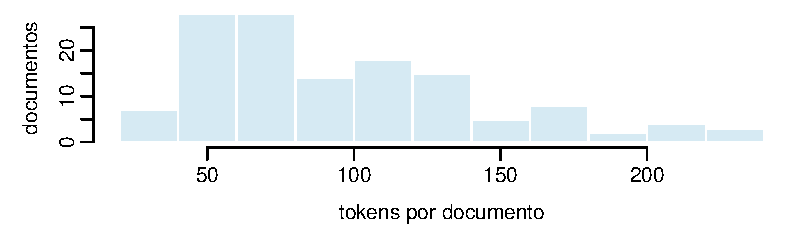
\includegraphics[width=0.48\linewidth]{figure/fig-tam-1} 

}


\end{knitrout}
  \fonte{Elaborada pelos autores.}
\end{figure}

\textbf{Termos mais frequentes.} Na tokenização bruta, os 10 termos mais
frequentes são \texttt{de} (910), \texttt{a} (494), \texttt{e} (392), \texttt{o} (365), \texttt{do} (301), \texttt{da} (250), \texttt{em} (226), \texttt{que} (157), \texttt{com} (126), \texttt{na} (114): todos os 10 são palavras funcionais vazias
de conteúdo temático, o que motivou o peso IDF e a remoção das 27
\textit{stopwords} na Aula~03 (reduzindo o vocabulário de 4.250 para 3.483
termos e revelando \texttt{santos}, \texttt{sao}, \texttt{cidade} e
\texttt{porto} no topo).

\begin{table}[!htb]
  \centering
  \caption{As três consultas de trabalho no corpus: documentos devolvidos, 1.º lugar e nDCG@5}
  \label{tab:busca}
  \small
  \begin{tabular}{@{}lrrccrrr@{}}
    \toprule
    Consulta de trabalho & AND & OR & 1.º Cosseno & 1.º BM25 & TF-IDF & Cosseno & BM25 \\
    \midrule
    1. \texttt{porto de santos}  & \text{21} & \text{85} & \texttt{d76} & \texttt{d76} & 0,87 & 1,00 & 1,00 \\
    2. \texttt{praias e turismo} & \text{6} & \text{22} & \texttt{d2} & \texttt{d80} & 0,72 & 0,70 & 0,51 \\
    3. \texttt{forte sao joao}   & \text{0} & \text{8} & \texttt{d117} & \texttt{d117} & 0,68 & 0,68 & 0,68 \\
    \midrule
    Tempo médio (ms) & 0,3 & 0,3 & & & 0,4 & 3,2 & 0,5 \\
    \bottomrule
  \end{tabular}
  \fonte{Elaborada pelos autores. nDCG@5 calculado com \texttt{qrels\_jorge\_2026-10-13.csv} \cite{jarvelin2002}.}
\end{table}

\textbf{Veredito.} A Tabela~\ref{tab:busca} comprova que o corpus responde às
três perguntas com alta precisão: em $q_1$, Cosseno e BM25 cravam \texttt{d76}
(inauguração do Porto de Santos em 1892) em 1.º lugar com $\text{nDCG@5} = 1,00$;
em $q_2$, o Cosseno coloca \texttt{d2} (praias do Guarujá) no topo e o BM25
promove \texttt{d80} e \texttt{d118}; em $q_3$, ambos posicionam \texttt{d117}
(Forte de São João em Bertioga) na liderança, validando o corpus para as etapas
de avaliação formal (Aula~5,5), Rocchio/PRF (Aula~06) e LSA/RRF (Aula~07).

\postextual
{\SingleSpacing\footnotesize
\bibliography{referencias}}

\end{document}
